\section{Exemples de grandeurs physiques}

\subsection{Liées au système solaire}

Les positions des planètes par rapport au soleil sont des grandeurs physiques. La masse du soleil est une grandeur physique. Les vitesses des planètes par rapport au soleil sont des grandeurs physiques.

\subsection{Liées à l'oscillateur harmonique}

La masse du mobile accroché au ressort est une grandeur physique ainsi que la raideur du ressort. Elle ne dépendent pas du temps (le temps est la grandeur physique affichée par une horloge).

\begin{center}
%https://physagreg.fr/schemas-figures-physique-svg-tikz.php
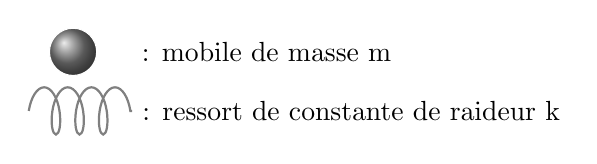
\begin{tikzpicture} [scale=0.75, decoration={coil,aspect=0.4,segment length=3mm,amplitude=3mm}]
%decoration : gère l'aspect du ressort par l'instruction decorate
\tikzset{ressort/.style={thick,gray,smooth}} %définition d'un style de ressort

\begin{scope}
\draw [rounded corners=4pt,color=white,ball color=gray,smooth] (0,-2.5) circle (0.4) node [right=0.75cm,black] {: mobile de masse m} ;
\draw[ressort,decorate,rotate=0] (-0.75,-3.5)--(1,-3.5) node [right=0cm,black] {: ressort de constante de raideur k};
\end{scope}
\end{tikzpicture} 

\end{center}

La longueur du ressort est une grandeur physique susceptible de dépendre du temps. 

\begin{center}
%https://physagreg.fr/schemas-figures-physique-svg-tikz.php
\begin{tikzpicture} [scale=0.75, decoration={coil,aspect=0.4,segment length=3mm,amplitude=3mm}]
%decoration : gère l'aspect du ressort par l'instruction decorate
\tikzset{ressort/.style={thick,gray,smooth}} %définition d'un style de ressort

\draw [dashed] (2,-4.5) --++ (4,0);
\draw node [left] at (2,-4.5) {O};
\draw [->] (2,-4.5) --++ (0,-2) node [left] {$x$};
\draw [dashed] (2,-5.5) --++ (4,0) ;
\draw node [left] at (2,-5.5) {$x(t)$} ;

%ressort
\begin{scope}
\draw[ressort,decorate] (0,-0.3)--(0,-3) ;
\draw[thick,gray] (0,0) -- (0,-0.3);
\fill [pattern=north east lines] (-0.5,0) rectangle (0.5,0.3); %bloc qui tient le ressort
\draw[thick] (-0.5,0) -- (0.5,0); %bloc qui tient le ressort
%fin ressort
\draw[line width=0.5pt,<->,>=triangle 45](-0.8,0) -- (-0.8,-3) node [midway,left] {$l_{\text{\bf 0}}$} ;
\end{scope}

\begin{scope}[xshift=3cm]%Décalage horizontale de 3 cm
\draw[ressort,decorate] (0,-0.3)--(0,-4) ;

%bloc qui tient le ressort
\draw[thick,gray] (0,0) -- (0,-0.3); \fill [pattern=north east lines] (-0.5,0) rectangle (0.5,0.3); \draw[thick](-0.5,0)--(0.5,0); %fin ressort

\draw[line width=0.5pt,<->,>=triangle 45](-0.8,0) -- (-0.8,-4.1) 
node [midway,left] {$l_{\text{\bf éq}}$} ;
\draw [thick](0,-4)--(0,-4.5);
\draw [rounded corners=4pt,color=white,ball color=gray,smooth] (0,-4.5) circle (0.4) ;

\draw [very thick,-latex] (0,-4.5)--++(0,-1.5) node [midway,right=0.25cm] {$\overrightarrow{P}$};
\draw [very thick,-latex] (0,-4.15)--(0,-2.9) 
node [midway,right=0.25cm] {$\overrightarrow{T_{\text{\bf éq}}}$};
\end{scope}

\begin{scope}[xshift=6cm]
\draw[ressort,decorate] (0,-0.3)--(0,-5) ;

%bloc qui tient le ressort
\draw[thick,gray] (0,0) -- (0,-0.3); \fill [pattern=north east lines] (-0.5,0) rectangle (0.5,0.3);
%pattern définit un style de remplissage de la forme
\draw[thick](-0.5,0)--(0.5,0); %fin ressort

\draw[line width=0.5pt,<->,>=triangle 45](-0.8,0) -- (-0.8,-5.1) node [midway,left] {$l(t)$} ;
\draw [thick](0,-5)--(0,-5.5);
\draw [rounded corners=4pt,color=white,ball color=gray,smooth] (0,-5.5) circle (0.4) ;

%rounded corners = coins arrondis de tant de points
%ball color = style de forme

\draw [very thick,-latex] (0,-5.5)--++(0,-1.5) node [midway,above=0.1cm,right=0.25cm] {$\overrightarrow{P}$};
\draw [very thick,-latex] (0,-5.15)--(0,-3.25) node [midway,right=0.25cm] {$\overrightarrow{T}$};
\end{scope}
\end{tikzpicture} 

\end{center}

Le poids et la tension du ressort sont des grandeurs physiques vectorielles (la masse du mobile et la raideur du ressort sont des grandeurs scalaires).

L'élongation du ressort $x(t)=l(t)-l_0$ est une grandeur physique.

%La masse du pendule simple, ainsi que sa longueur sont des grandeurs physique

\subsection{Liées à un gaz}

La température du gaz enfermé dans une enceinte est une grandeur physique. Ainsi que son volume, sa pression, son nombre de particules le constituant.

%Un verre d'eau avec des glaçons définie un système tehrmodynamique. Le système est l'eau liquide et les glaçons.

